
\section{Submodularity in Weighted Constraint Reasoning}
  Many application require efficient representation and reasoning about factors like fuzziness, probabilities, preferences, and/or costs. Various extensions to the basic framework of Constraint Satisfaction Problems (CSPs) \cite{D:BOOK:03} have been introduced to incorporate and reason about such ``soft'' constraints. These include variants like \emph{fuzzy-CSPs}, \emph{probabilistic-CSPs}, and Weighted-CSPs (WCSPs). A WCSP is an \emph{optimization} version of a CSP in which the constraints are no longer ``hard,'' but are extended by associating (non-negative) \emph{costs} with the tuples. The goal is to find an assignment of values to all variables from their respective domains such that the total cost is \emph{minimized}.
  
  For simplicity, we restrict ourselves to Boolean WCSPs. Note that this class can be used to model important combinatorial problems such as representing and reasoning about user preferences \cite{BBDHP:JAIR:04}, over-subscription planning with goal preferences \cite{D:IJCAI:07}, combinatorial auctions \cite{S:AI:02}, and bioinformatics \cite{SGSST:AI:07}, energy minimization problems in probabilistic settings, computer vision, Markov Random Fields \cite{K:MSR:05}, etc. In addition, many real-world domains exhibit \emph{submodularity} in the cost structure that is worth exploiting for computational benefits. In what follows, we define a class of submodular constraints over Boolean domains and give a polynomial-time algorithm for solving instances from this class. 
  
\subsection{Weighted Constraint Satisfaction Problems}
  Formally, a WCSP is defined by a triplet $\langle \mathcal{X,D,C} \rangle$ where $\mathcal{X} = \{ X_1,X_2 \ldots X_N \}$ is a set of \emph{variables}, and $\mathcal{C} = \{ C_1,C_2 \ldots C_M \}$ is a set of \emph{weighted constraints} on subsets of the variables. Each variable $X_i$ is associated with a discrete-valued \emph{domain} $D_i \in \mathcal{D}$, and each constraint $C_i$ is defined on a certain subset $S_i \subseteq \mathcal{X}$ of the variables. $S_i$ is referred to as the \emph{scope} of $C_i$; and $C_i$ specifies a non-negative \emph{cost} for every possible combination of values to the variables in $S_i$. The \emph{arity} of the constraint $C_i$ is equal to $|S_i|$. An \emph{optimal} solution is an assignment of values to all variables (from their respective domains) so that the \emph{sum} of the costs (as specified locally by each weighted constraint) is \emph{minimized}. In a Boolean WCSP, the size of any variable's domain is $2$ (that is, $D_i = \{ 0,1 \}$ for all $i$). Boolean WCSPs are representationally as powerful as WCSPs; and it is well known that optimally solving Boolean WCSPs is NP-hard in general \cite{D:BOOK:03}. The \emph{constraint graph} associated with a WCSP instance is an undirected graph where a node represents a variable and an edge $(X_i,X_j)$ exists if and only if $X_i$ and $X_j$ appear together in some constraint.


\subsection{Submodular Constraints}
  Submodular constraints over Boolean domains correspond directly to \emph{submodular set functions}. A set function $\psi : 2^V \rightarrow \mathrm{Q}$ defined on all subsets of a set $V$ is \emph{submodular} if and only if, for all subsets $S, T \subseteq V$, we have $\psi(S \cup T) + \psi(S \cap T) \leq \psi(S) + \psi(T)$. A submodular constraint is a weighted constraint with a submodular cost function. Here, the correspondence is in light of the observation that any subset $S$ can be interpreted as specifying the Boolean variables in $V$ that are set to $1$. Boolean WCSPs with submodular constraints are known to be tractable \cite{ZSH:CSC:10}. However, the general algorithm for solving Boolean WCSPs with submodular constraints has a time complexity of $O(N^6)$, which is not very practical. Specific classes of submodular constraints have been shown to be related to graph cuts, and are therefore solvable more efficiently \cite{ZSH:CSC:10}.

\subsection{Lifted Graphical Representations for Weighted Constraints}
  \emph{Constraint Composite Graphs} (CCGs) are combinatorial structures associated with optimization problems posed as WCSPs. They provide a unifying framework for exploiting both the \emph{graphical} structure of the variable interactions as well as the \emph{numerical} structure of the weighted constraints \cite{K:CP:08}. We reformulate WCSPs as \emph{minimum weighted vertex cover} problems to construct simple bipartite graph representations for important classes of submodular constraints, thereby translating them into max-flow problems on bipartite graphs.

  The concept of the minimum weighted VC\footnote{A \emph{vertex cover} (VC) is a set of nodes $S$ such that every edge has at least one end point in $S$.} on a given undirected graph $G=\langle V,E \rangle$ can be \emph{extended} to the notion of projecting minimum weighted VCs onto a given IS\footnote{$U$ is an \emph{independent set} (IS) of a graph if and only if no two nodes in $U$ are connected by an edge.} $U \subseteq V$. The input to such a projection is the graph $G$ as well as an identified IS $U=\{u_1, u_2 \ldots u_k\}$. The output is a \emph{table} of $2^k$ numbers. Each entry in this table corresponds to a $k$-bit vector. We say that a $k$-bit vector imposes the following restrictions: if the $i^{th}$ bit is $0$ ($1$), the node $u_i$ is necessarily excluded (included) from the minimum weighted VC. The value of an entry is the weight of the minimum weighted VC \emph{conditioned} on the restrictions imposed by it. Figure \ref{VC_example} presents a simple example.
  
\begin{figure}[t]
  \centering
  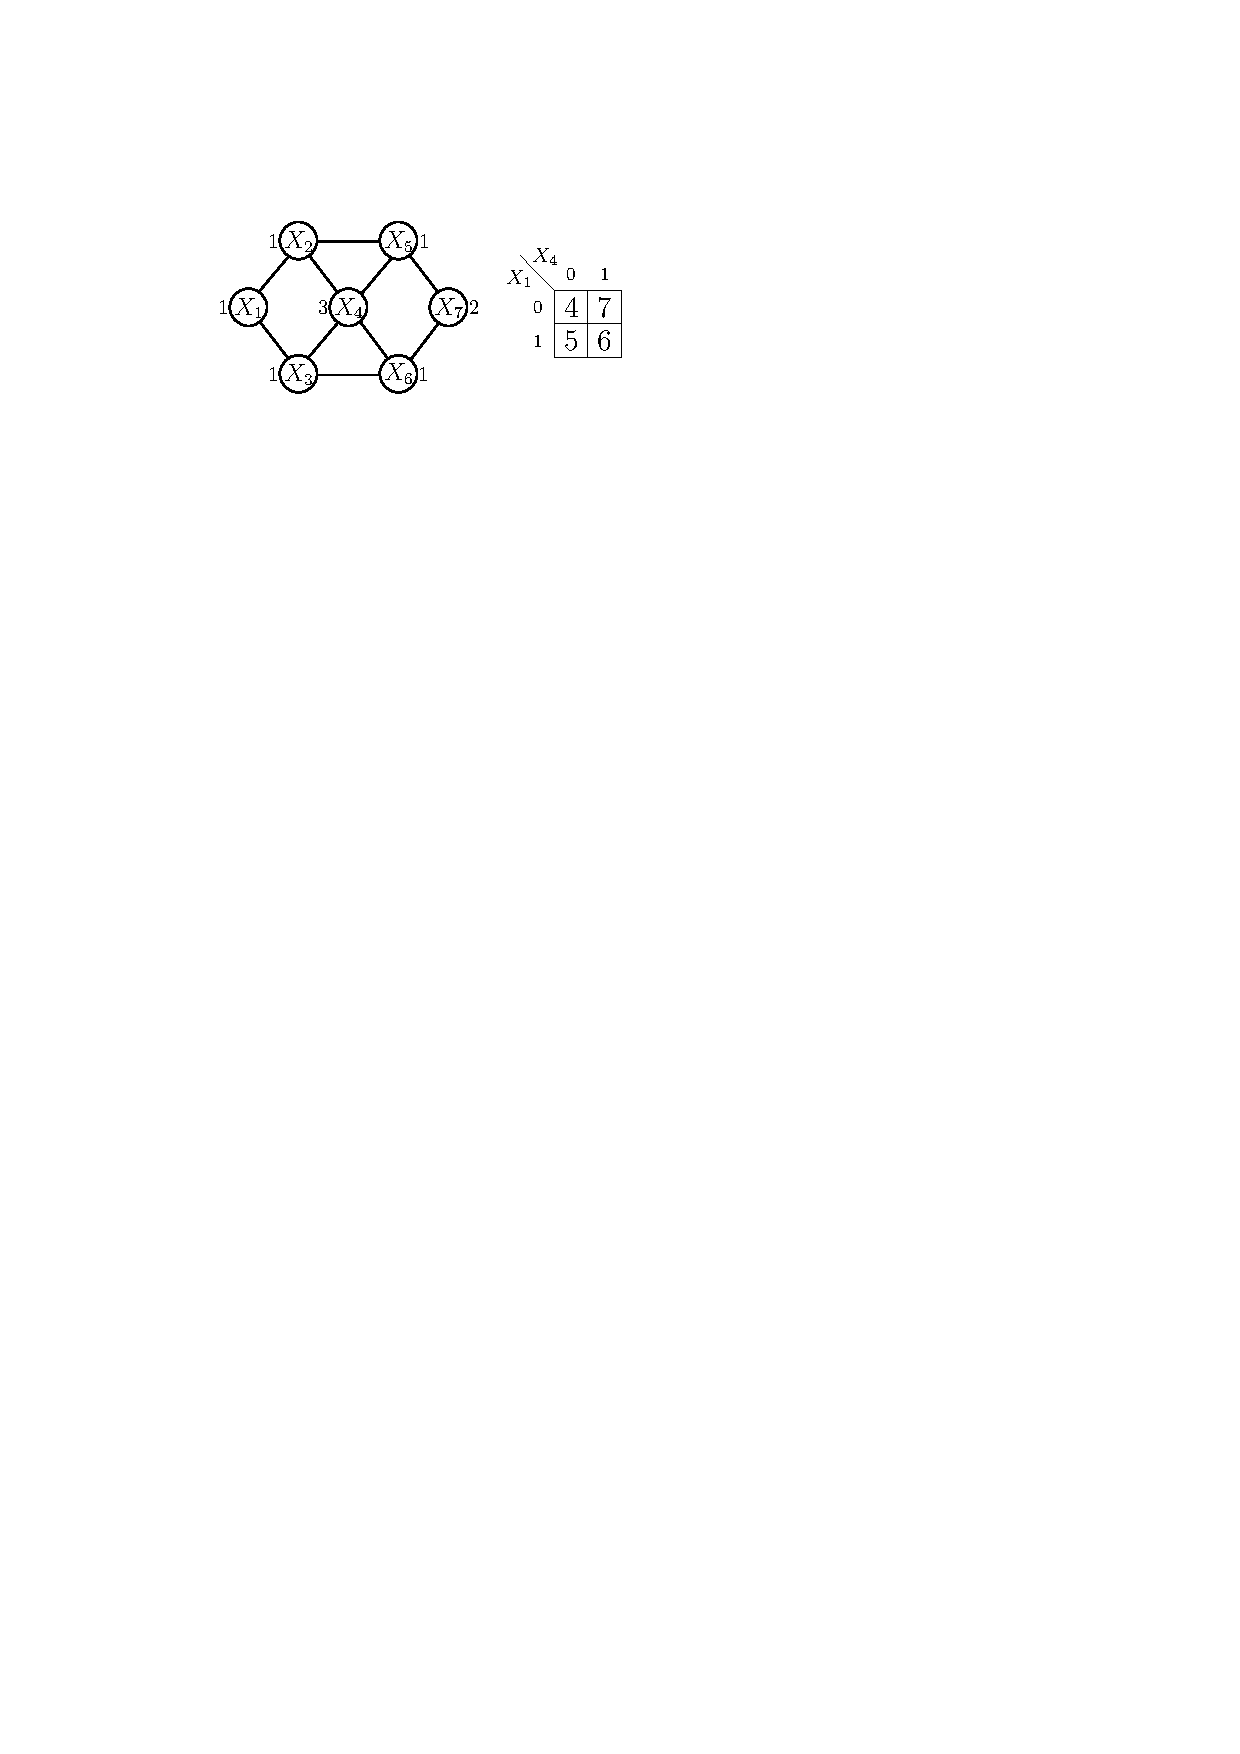
\includegraphics[width=0.35\textwidth]{figs/fig5}
  \caption{The table on the right-hand side represents the projection of the minimum weighted VC problem onto the IS $\{ X_1, X_4 \}$ of the node-weighted undirected graph on the left-hand side. (The weights on $X_4$ and $X_7$ are set to $3$ and $2$, respectively, while all other nodes have unit weights.) The entry `$7$' in the cell $(X_1=0, X_4=1)$, for example, indicates that, when $X_1$ is prohibited from being in the minimum weighted VC but $X_4$ is necessarily included in it, then the weight of the minimum weighted VC - $\{ X_2, X_3, X_4, X_7 \}$ or $\{ X_2, X_3, X_4, X_5, X_6 \}$ - is $7$.}
  \label{VC_example}
\end{figure}

  The aformentioned table can be viewed as a weighted constraint over $|U|$ Boolean variables. Conversely, given a (Boolean) weighted constraint, we can think about designing a ``lifted'' representation for it so as to be able to view it as the projection of a minimum weighted VC problem in some node-weighted undirected graph. This idea was first discussed in \cite{K:ISAIM:08}. The benefit of constructing these graphical representations for individual constraints lies in the fact that the ``lifted'' graphical representation for the entire WCSP can be obtained simply by ``merging\footnote{nodes that represent the same variable are simply ``merged'' - along with their edges - and every ``composite'' node is given a weight equal to the sum of the individual weights of the merged nodes.}'' them. This ``merged'' graph is referred to as the CCG associated with the WCSP. Computing the minimum weighted VC for the CCG yields a solution for the WCSP; namely, if $X_i$ is in the minimum weighted VC, then it is assigned the value $1$ in the WCSP, else it is assigned the value $0$ in the WCSP. Figure \ref{VC_example} shows an example WCSP and its CCG.
  
\begin{figure}[t]
  \centering
  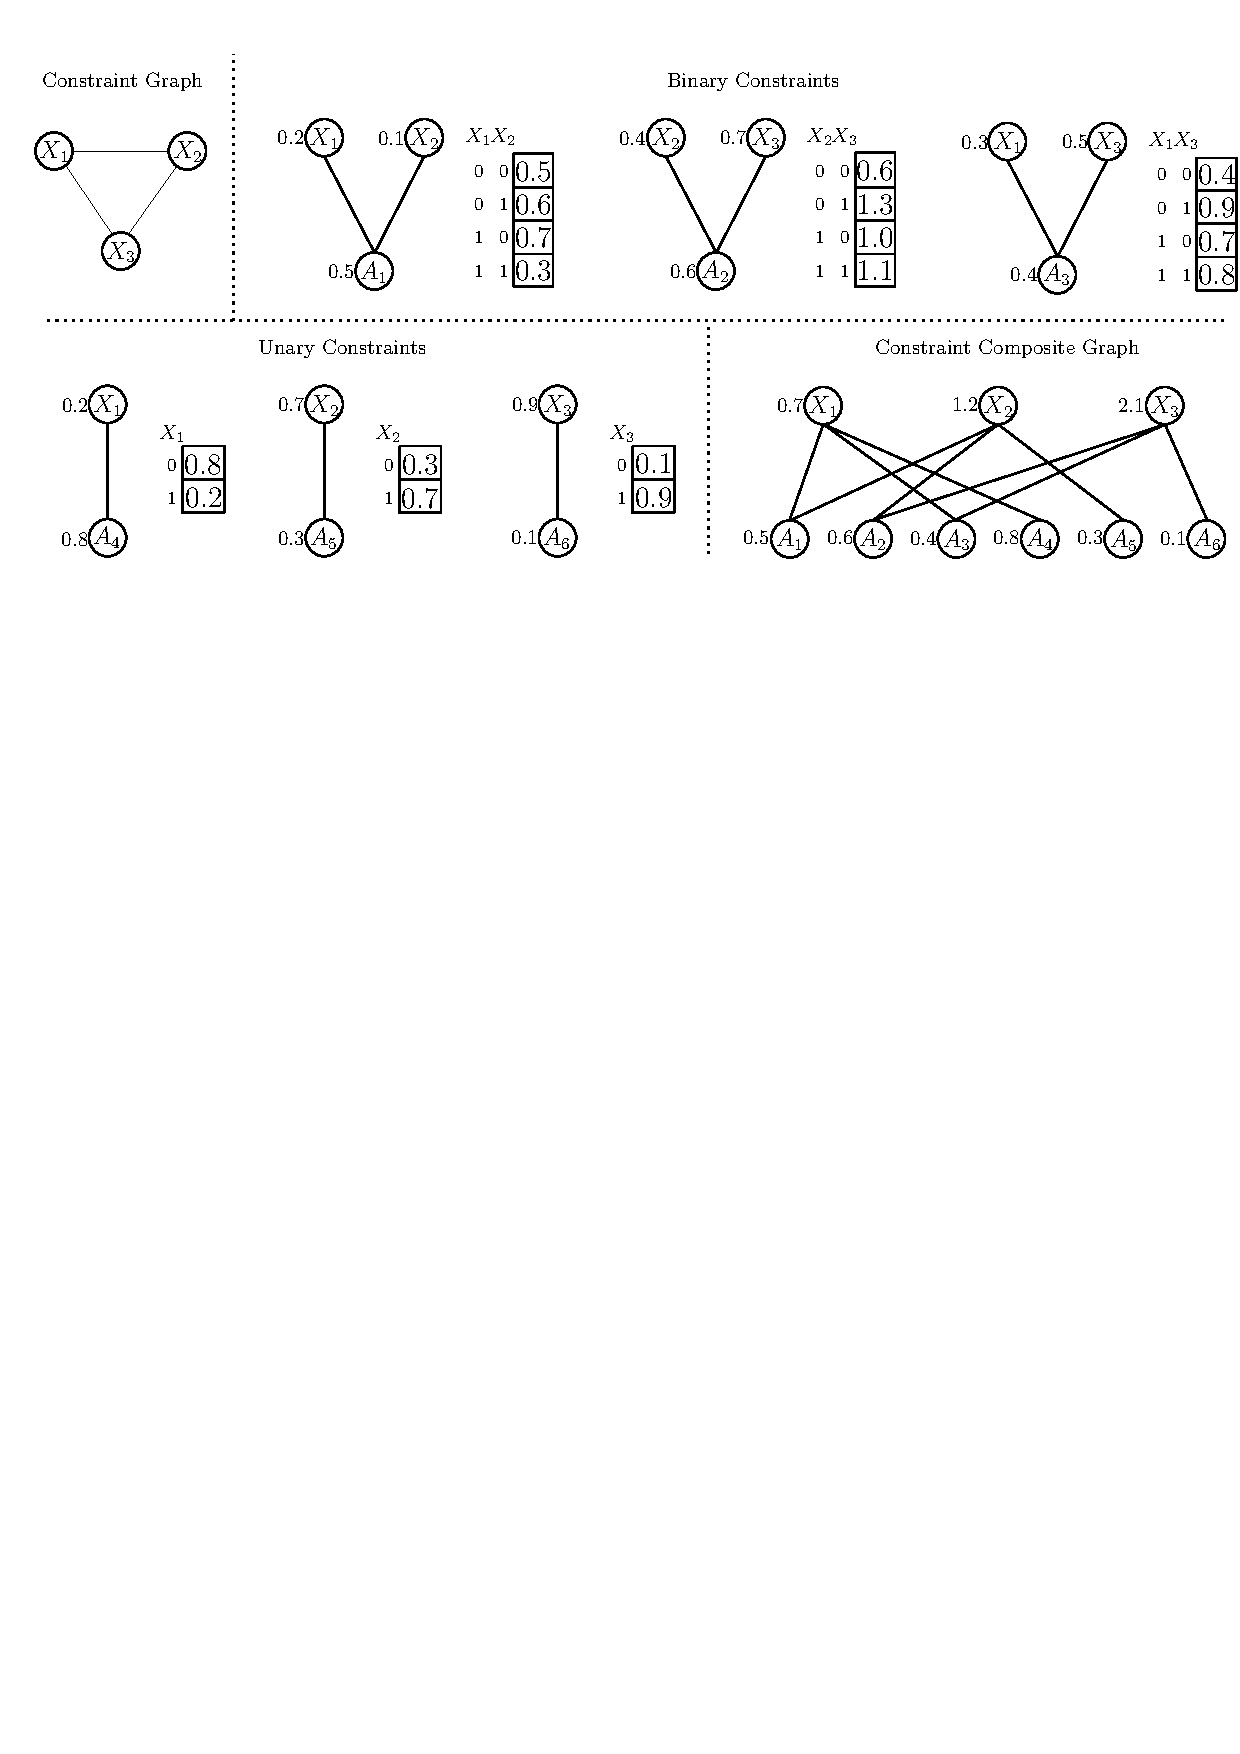
\includegraphics[width=0.9\textwidth]{figs/fig7}
  \caption{Shows a WCSP over $3$ Boolean variables. The constraint network is shown in the top-left cell, and the $6$ binary and unary weighted constraints are shown along with their lifted graphical representations in the $1^{st}$ and $2^{nd}$ rows. The CCG is shown in the bottom-right cell.}
  \label{ccg_example}
\end{figure}

  Any given weighted constraint on Boolean variables can be represented graphically using a \emph{tripartite} graph, which can be constructed in polynomial time \cite{K:CP:08}. In many cases, the lifted graphical representations even turn out to be only \emph{bipartite}. Since the resulting CCG is also bipartite if each of the individual graphical representations are bipartite, the tractability of the language $\mathcal{L}_{bipartite}^{Boolean}$ - the language of all Boolean weighted constraints with a bipartite graphical representation - is readily established. This is because solving minimum weighted VC problems on bipartite graphs is reducible to max-flow problems, and can therefore be solved efficiently in polynomial time.
  
  Finally, Boolean weighted constraints can be represented as multivariate polynomials on the variables participating in that constraint \cite{ZSH:CSC:10,K:CP:08}. The coefficients of the polynomial can be computed with a standard Gaussian Elimination procedure for solving systems of linear equations. The linear equations themselves arise from substituting different combinations of values to the variables, and equating them to the corresponding entries in the weighted constraint. One way to build the CCG of a given weighted constraint is: (a) build the graphical representations for each of the individual terms in the multivariate polynomial; and (b) ``merge'' these graphical representations \cite{K:CP:08}.

\subsection{Submodular Constraints with bounded arity}
  The focus of \cite{KCK:SARA:13} is on bounded arity submodular constraints (that is, submodular constraints with arity at most $K$, for some constant $K$) and providing asymptotically improved algorithms for solving them. The reason these submodular constraints can be solved more efficiently is because the underlying max-flow problems are staged on bipartite graphs. For Boolean WCSPs with arity at most $K$, the bipartite CCG has $N$ nodes in one partition, at most $2^K M$ nodes in the other partition, and at most $K 2^K M$ edges. For $K$ bounded by a constant, this results in a time complexity of $O(N M \log M)$. This significantly improves on the $O((N+M)^{3})$ time complexity of the algorithm provided by \cite{ZSH:CSC:10}.\footnote{For arity $K$, $M$ could be as large as $N \choose K$.} Figure \ref{fig_lifted_rep} shows the lifted graphical representation for all possible terms of a constraint of arity $3$.
  
\begin{figure}[t]
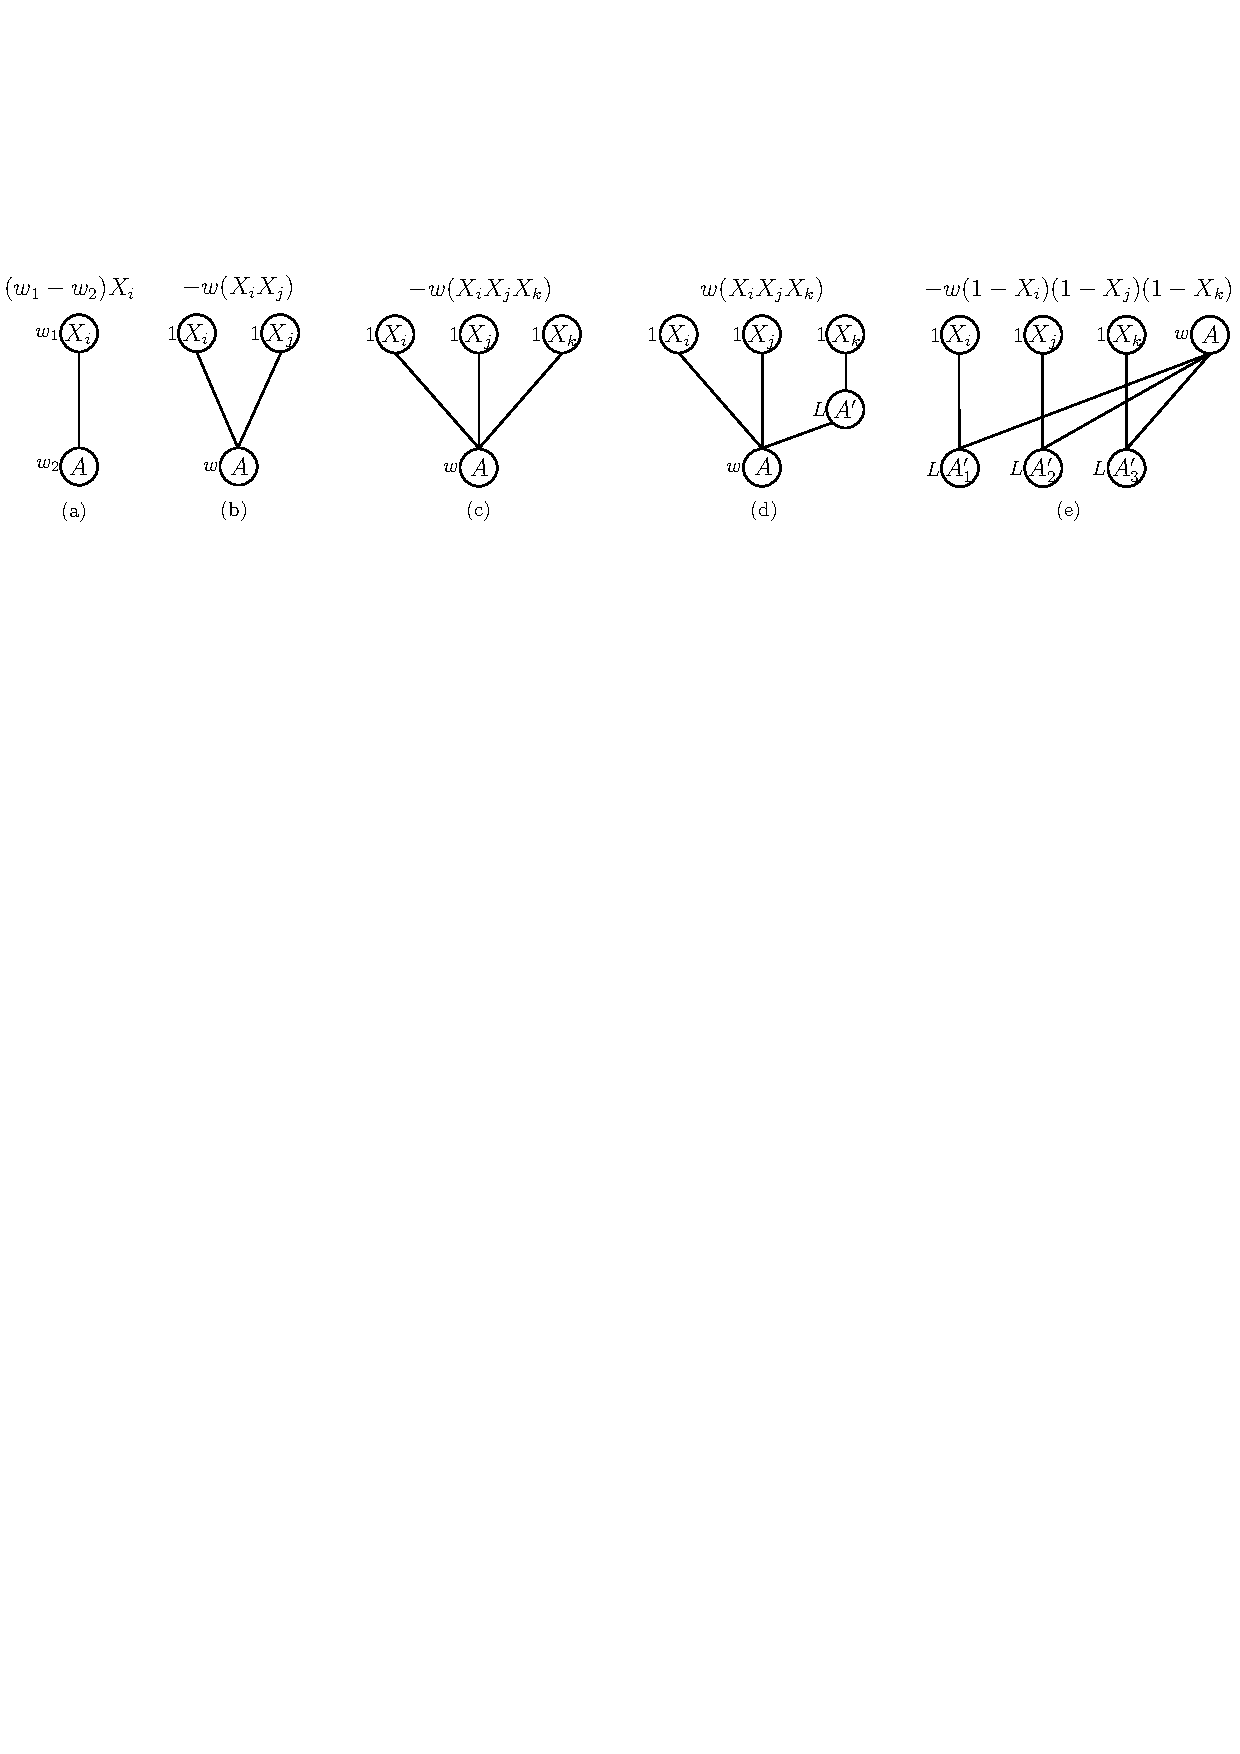
\includegraphics[width=\textwidth]{figs/fig8.pdf}
\caption{Lifted graphical representations for different kind of terms. (a) represents a linear term, either positive or negative, where $w_1$ and $w_2$ are chosen appropriately. (b) represents a negative quadratic term. (c) represents a negative cubic term. (d) illustrates the ``change of variable'' method and essentially represents a leading positive cubic term. (e) is the same ``flower'' structure shown in (c), but with a ``thorn'' introduced for each variable. The resulting graph is also bipartite, because the auxiliary variable $A$ can be moved to the same partition as the original variables. The graph now represents the term $-w (1-X_i)(1-X_j)(1-X_k)$, which in effect, is a bipartite representation for an expression with a leading positive cubic term.}
\label{fig_lifted_rep}
\end{figure}
